% Chapter Template

\chapter{Descripci\'on t\'ecnica} % Main chapter title

\label{Chapter3} % Change X to a consecutive number; for referencing this chapter elsewhere, use \ref{ChapterX}

%----------------------------------------------------------------------------------------
%	SECTION 1
%----------------------------------------------------------------------------------------

\section{Descripci\'on t\'ecnica}

\subsection{Aspectos t\'ecnicos de relevancia para los usuarios}
La aplicaci\'on m\'ovil funcionar\'a en dispositivos con Android 5.0, la aplicaci\'on web funcionar\'a en los navegadores Firefox y Chrome. Se necesitar\'a conexi\'on a Internet excepto en el caso de canciones descargadas en la aplicaci\'on m\'ovil. 
\subsection{Aspectos t\'ecnicos de relevancia para el cliente}
El backend del sistema se entregar\'a con m\'aquinas virtuales funcionando en un cl\'uster privado a modo de demostraci\'on, las m\'aquinas ser\'an maquinas KVM montadas sobre Debian y con un sistema Debian invitado. El cl\'uster de demostraci\'on contar\'a con un almacenamiento bruto de 20GB, un total de 5 maquinas virtuales simulando las 5 m\'aquinas f\'isicas y en una de ellas se virtualizar\'a el servidor backend y la base de datos
Adem\'as se entregar\'an las instrucciones del montaje y despliegue as\'i como recomendaciones y observaciones tanto de hardware como se software para poder montar un sistema real sobre hierro en el cl\'uster privado del cliente.
Adem\'as se entregar\'a el c\'odigo de la aplicaci\'on m\'ovil, de la aplicaci\'on web y del servidor web asi como cualquier otro software necesario.

\subsection{Descripci\'on t\'ecnica preliminar}
El sistema cuenta con 4 componentes principales: una aplicaci\'on Android, una aplicaci\'on web, un servidor web (a modo de coordinaci\'on) y un sistema de almacenamiento.
El servidor web ser\'a una sola m\'aquinas con sistema operativo ProxmoxVE(basado en Debian), contar\'a con 2 m\'aquinas virtuales, una con PostgreSQL para la base de datos y otra con la aplicaci\'on backend en Tomcat. Ambas m\'aquinas almacenadas en el servicio de almacenamiento mediante RBD. Esto permite garantizar la integridad de los datos mediante replicaci\'on y en el caso de varias m\'aquinas permitir configurar HA para levantar las m\'aquinas en caso de ca\'ida.
El servicio de almacenamiento ser\'a un conjunto de 4 m\'aquinas, 3 ceph-nodes que ofrecen el almacenamiento, replica, distribuci\'on y consistencia de los datos y una cuarta, ceph\_rados\_gw que ofrece una interfaz REST mediante HTTP para el acceso a los datos equiparable a Amazon S3 o Swift. Adem\'as, todas las canciones y datos disponen de un URI.
Las comunicaciones con el cliente se realizar\'an siempre mediante HTTP con una interfaz RESTfull. El cliente se comunicar\'a con la aplicaci\'on Tomcat en caso de necesitar consultar valores o actualizar la base de datos y en cambio se comunicar\'a directamente con el servidor RADOS para obtener las canciones, esta separaci\'on permite no sobrecargar al servidor de Tomcat ni a su red con descargas de datos pesados.
Para soportar la integridad de los datos, el servicio de almacenamiento con 3 m\'aquinas permite una ca\'ida de 1 m\'aquina simultanea sin p\'erdida de servicio.

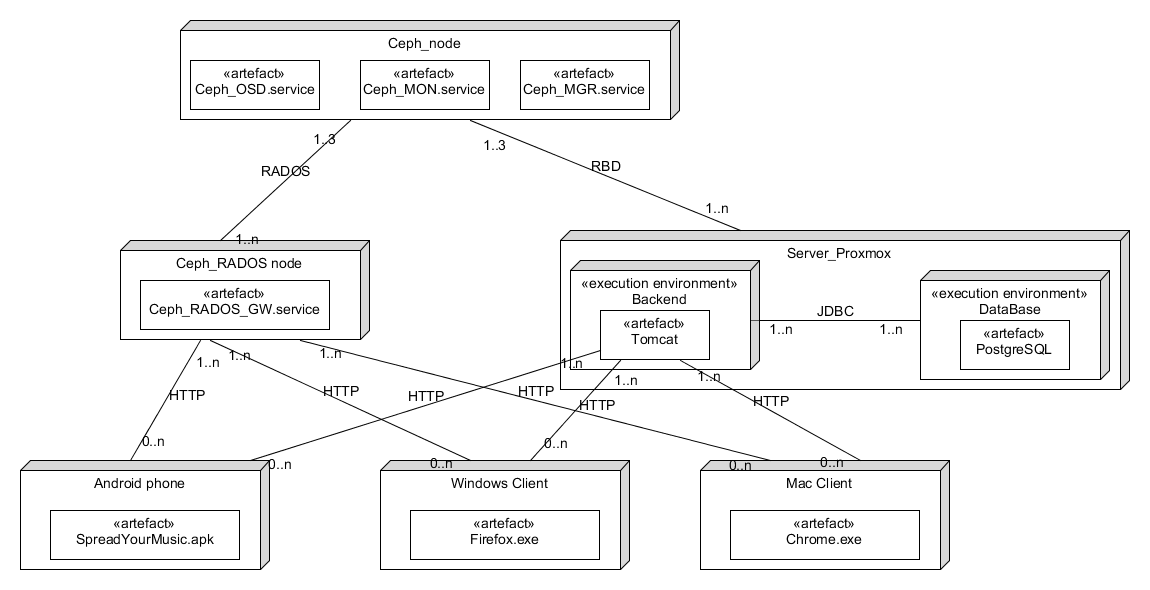
\includegraphics[width=6cm]{Figures/deployment.png}